
\begin{quote}
\noindent {\em These notes extend our ideas of linear advection to a scalar nonlinear equation.}
\end{quote}


\section{Burgers' equation}

The inviscid Burgers' equation is the simplest nonlinear hyperbolic
equation:
\begin{equation}
u_t + u u_x = 0
\end{equation}
Here $u$ is both the quantity being advected and the speed at which 
it is moving.
In conservative form, this appears as:
\begin{equation}
u_t + \left [\tfrac{1}{2} u^2 \right ]_x = 0
\end{equation}

The solution of this follows the same methodology as outlined above.
The interface states are predicted as:
\begin{eqnarray}
u^{n+1}_{i+1/2,L} &=& u^n_i + \frac{\Delta x}{2} \frac{\partial u}{\partial x}
                        + \frac{\Delta t}{2} \frac{\partial u}{\partial t} + \ldots \\
                &=& u^n_i + \frac{\Delta x}{2} \frac{\partial u}{\partial x}
                        + \frac{\Delta t}{2} \left (-u_i \frac{\partial u}{\partial x} \right ) + \ldots \\
                &=& u^n_i + \frac{\Delta x}{2} \left ( 1 - \frac{\Delta t}{\Delta x}u_i \right ) \frac{\partial u}{\partial x} + \ldots
\end{eqnarray}
The only difference with the linear advection equation is that now
$u_i \Delta t/\Delta x$ varies from zone to zone, whereas with linear
advection, it is the constant $C$.  The slopes are computed using
the same limiters as with linear advection.

The Riemann problem differs from linear advection.  It remains the
case that the solution is constant along the lines $x = ut + x_0$ (the
characteristics), but now those lines are no longer parallel.  If the
characteristic lines intersect, then there it is not possible to trace
backward from time to learn where the flow originated.  This is the 
condition for a {\em shock}.

Shock speed from jump conditions

Riemann problem
\begin{eqnarray}
\mathrm{if~} u_l > u_r:&& u_s = \left \{ \begin{array}{cl}
                u_l & \mathrm{if~} S > 0 \\ 
                u_r & \mathrm{if~} S < 0 \\
                0   & \mathrm{if~} S = 0 \end{array} \right .   \\[1em]
%
\mathrm{otherwise:}&& u_s = \left \{ \begin{array}{clc}
                u_l & \mathrm{if~} u_l \ge 0 \\  
                u_r & \mathrm{if~} u_r \le 0 \\  
                0   & \mathrm{otherwise} \end{array} \right .   
\end{eqnarray}
               
Once the interface states are constructed, the flux is calculated as:
\begin{equation}
F^{n+1/2}_{i+1/2} = \frac{1}{2} \left (u_{i+1/2}^{n+1/2} \right )^2
\end{equation}
and the conservative update is
\begin{equation}
u_i^{n+1} = u_i^n + \frac{\Delta t}{\Delta x} 
   \left ( F_{i-1/2}^{n+1/2} - F_{i+1/2}^{n+1/2} \right )
\end{equation}

The timestep constraint now must consider the most restrictive Courant 
condition over all the zones:
\begin{equation}
\Delta t = \min_i \left \{ \Delta x / u_i \right \}
\end{equation}


\begin{figure}[t]
\centering
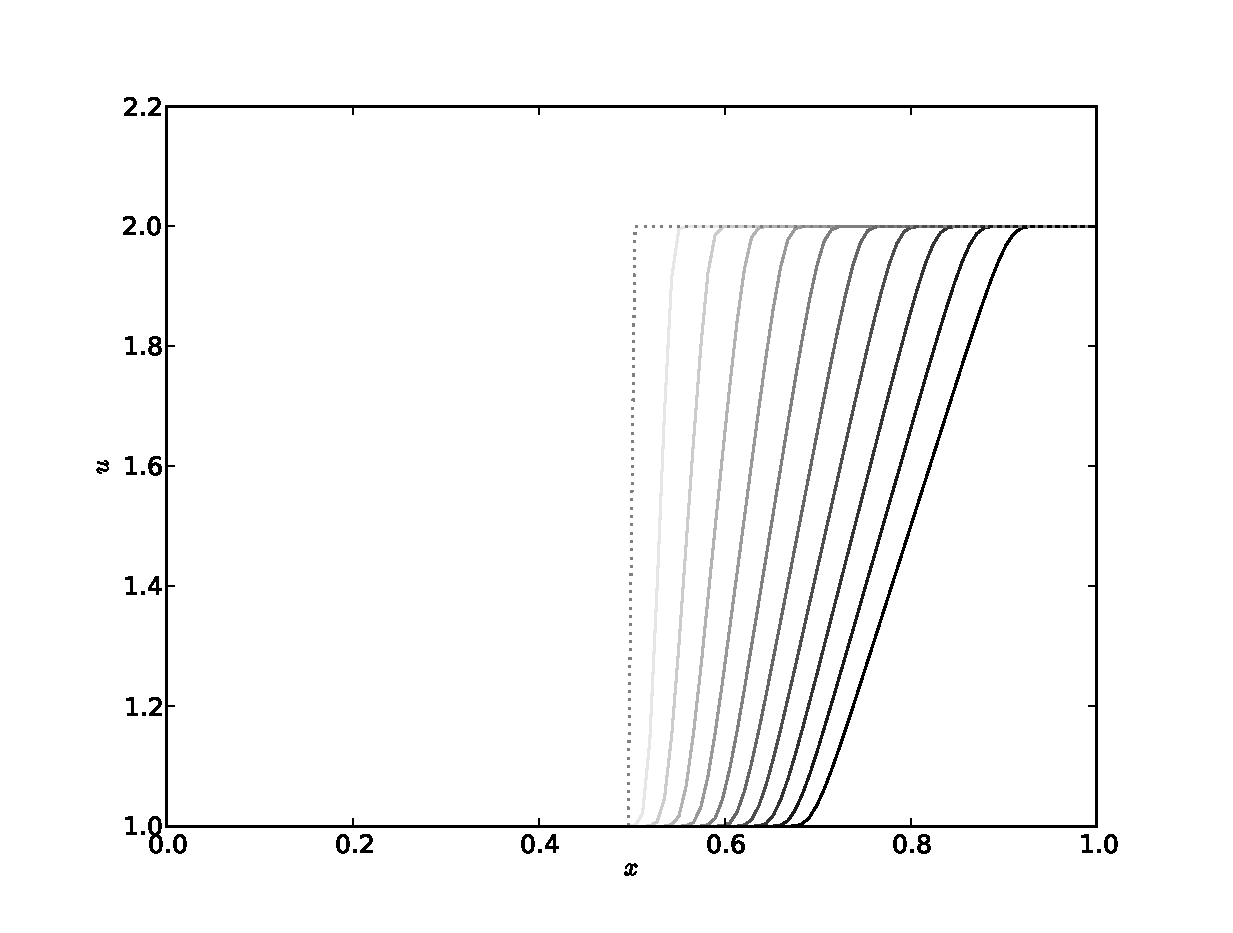
\includegraphics[width=3.0in]{fv-burger-rarefaction}
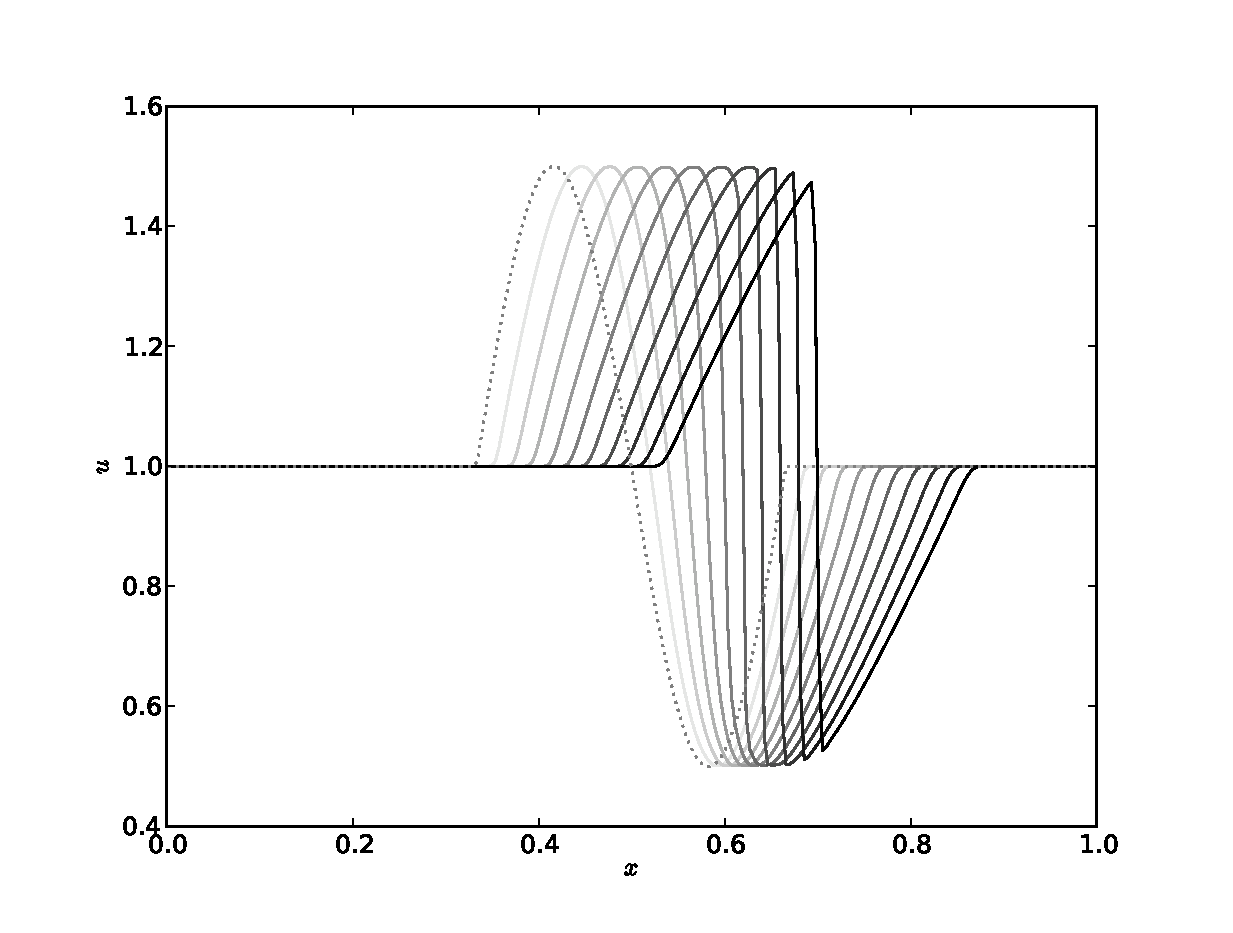
\includegraphics[width=3.0in]{fv-burger-sine}
\caption[Solutions to the inviscid Burgers'
  equation.]{\label{fig:burgers} Solution to the inviscid Burgers'
  equation with 256 zones and a Courant number, $C = 0.8$.  On the
  left, is a rarefaction---the left half of the domain was initialized
  with $u = 1$ and the right half with $u = 2$, creating a divergent
  flow.  On the right is a sine-wave steepening into a shock.  The
  curves are shown 0.02~s apart.}
\end{figure}

Figure~\ref{fig:burgers} shows the solution for two cases: a rarefaction
and a sine-wave steepening into a shock, using a piecewise linear
reconstruction and the MC limiter.


\section{Going further}
